\chapter{Introduction}

The increasing use of small unmanned aerial vehicles (UAVs) creates new challenges for aviation safety, especially in low-altitude airspace where helicopters frequently operate. Helicopters are commonly used for rescue missions, police operations, infrastructure inspection, and medical transport. In such environments, drones can become safety-critical obstacles because they may not carry transponders, and may be difficult to detect visually under adverse lighting, cluttered backgrounds, or high pilot workload. Detect-and-avoid (DAA) systems therefore require robust onboard perception methods that can detect, track, and predict the motion of such intruders early enough to support collision avoidance decisions \cite{fasano2016senseAvoid,skowron2019senseAvoidSmallUAS,riedel2025daaStandards}.

An onboard DAA system must perceive the surrounding airspace independently of information transmitted by the intruder. Camera sensors can provide valuable appearance information, but the depth and relative position of a small object may be difficult to estimate reliably at long distances or under unfavorable illumination. Light detection and ranging (LiDAR) offers a complementary sensing principle by actively measuring the distance to surrounding surfaces and representing them as three-dimensional point clouds. This direct geometric information is particularly relevant for DAA because collision-risk assessment depends not only on recognizing an intruder, but also on determining its position and motion relative to the host aircraft. LiDAR has therefore been extensively investigated as a sensing modality for the detection and tracking of small UAVs \cite{hammer2018potentialLidarUAV,hammer2018lidarSmallUAVs,dogru2022sparseLidarDrone}.

The use of LiDAR from an airborne platform nevertheless introduces substantial challenges. Both the host aircraft and the intruding drone may move independently, so that the sensor viewpoint, background, and observation geometry change continuously. Further more at increasing distance, a small drone may generate only a few intermittent LiDAR returns, making individual detections uncertain and requiring information to be combined over time. Reliable DAA consequently requires more than object detection in isolated sensor frames. The observations must be transformed into consistent coordinate systems, associated across time, and used to estimate the intruder's relative position and velocity despite sensor noise, ego-motion, incomplete measurements, and processing delay. The quality of this estimated state is critical for the safety of helicopter - UAV encounters.

This PhD project investigates how airborne RGB and LiDAR sensing can support the detection, and tracking of small non-cooperative drones for helicopter-oriented DAA. The research is structured as three consecutive stages. First, a real-world airborne RGB--LiDAR dataset will be developed to enable reproducible encounter evaluation. Second, this benchmark will be used to identify and address limitations in the detection and tracking of UAVs to develop a precise and efficient data-driven detection model. Third, the resulting perception outputs will be incorporated into a DAA evaluation framework to assess helicopter safety and initiate avoidance maneuvers.


\begin{figure}[htbp]
    \centering
    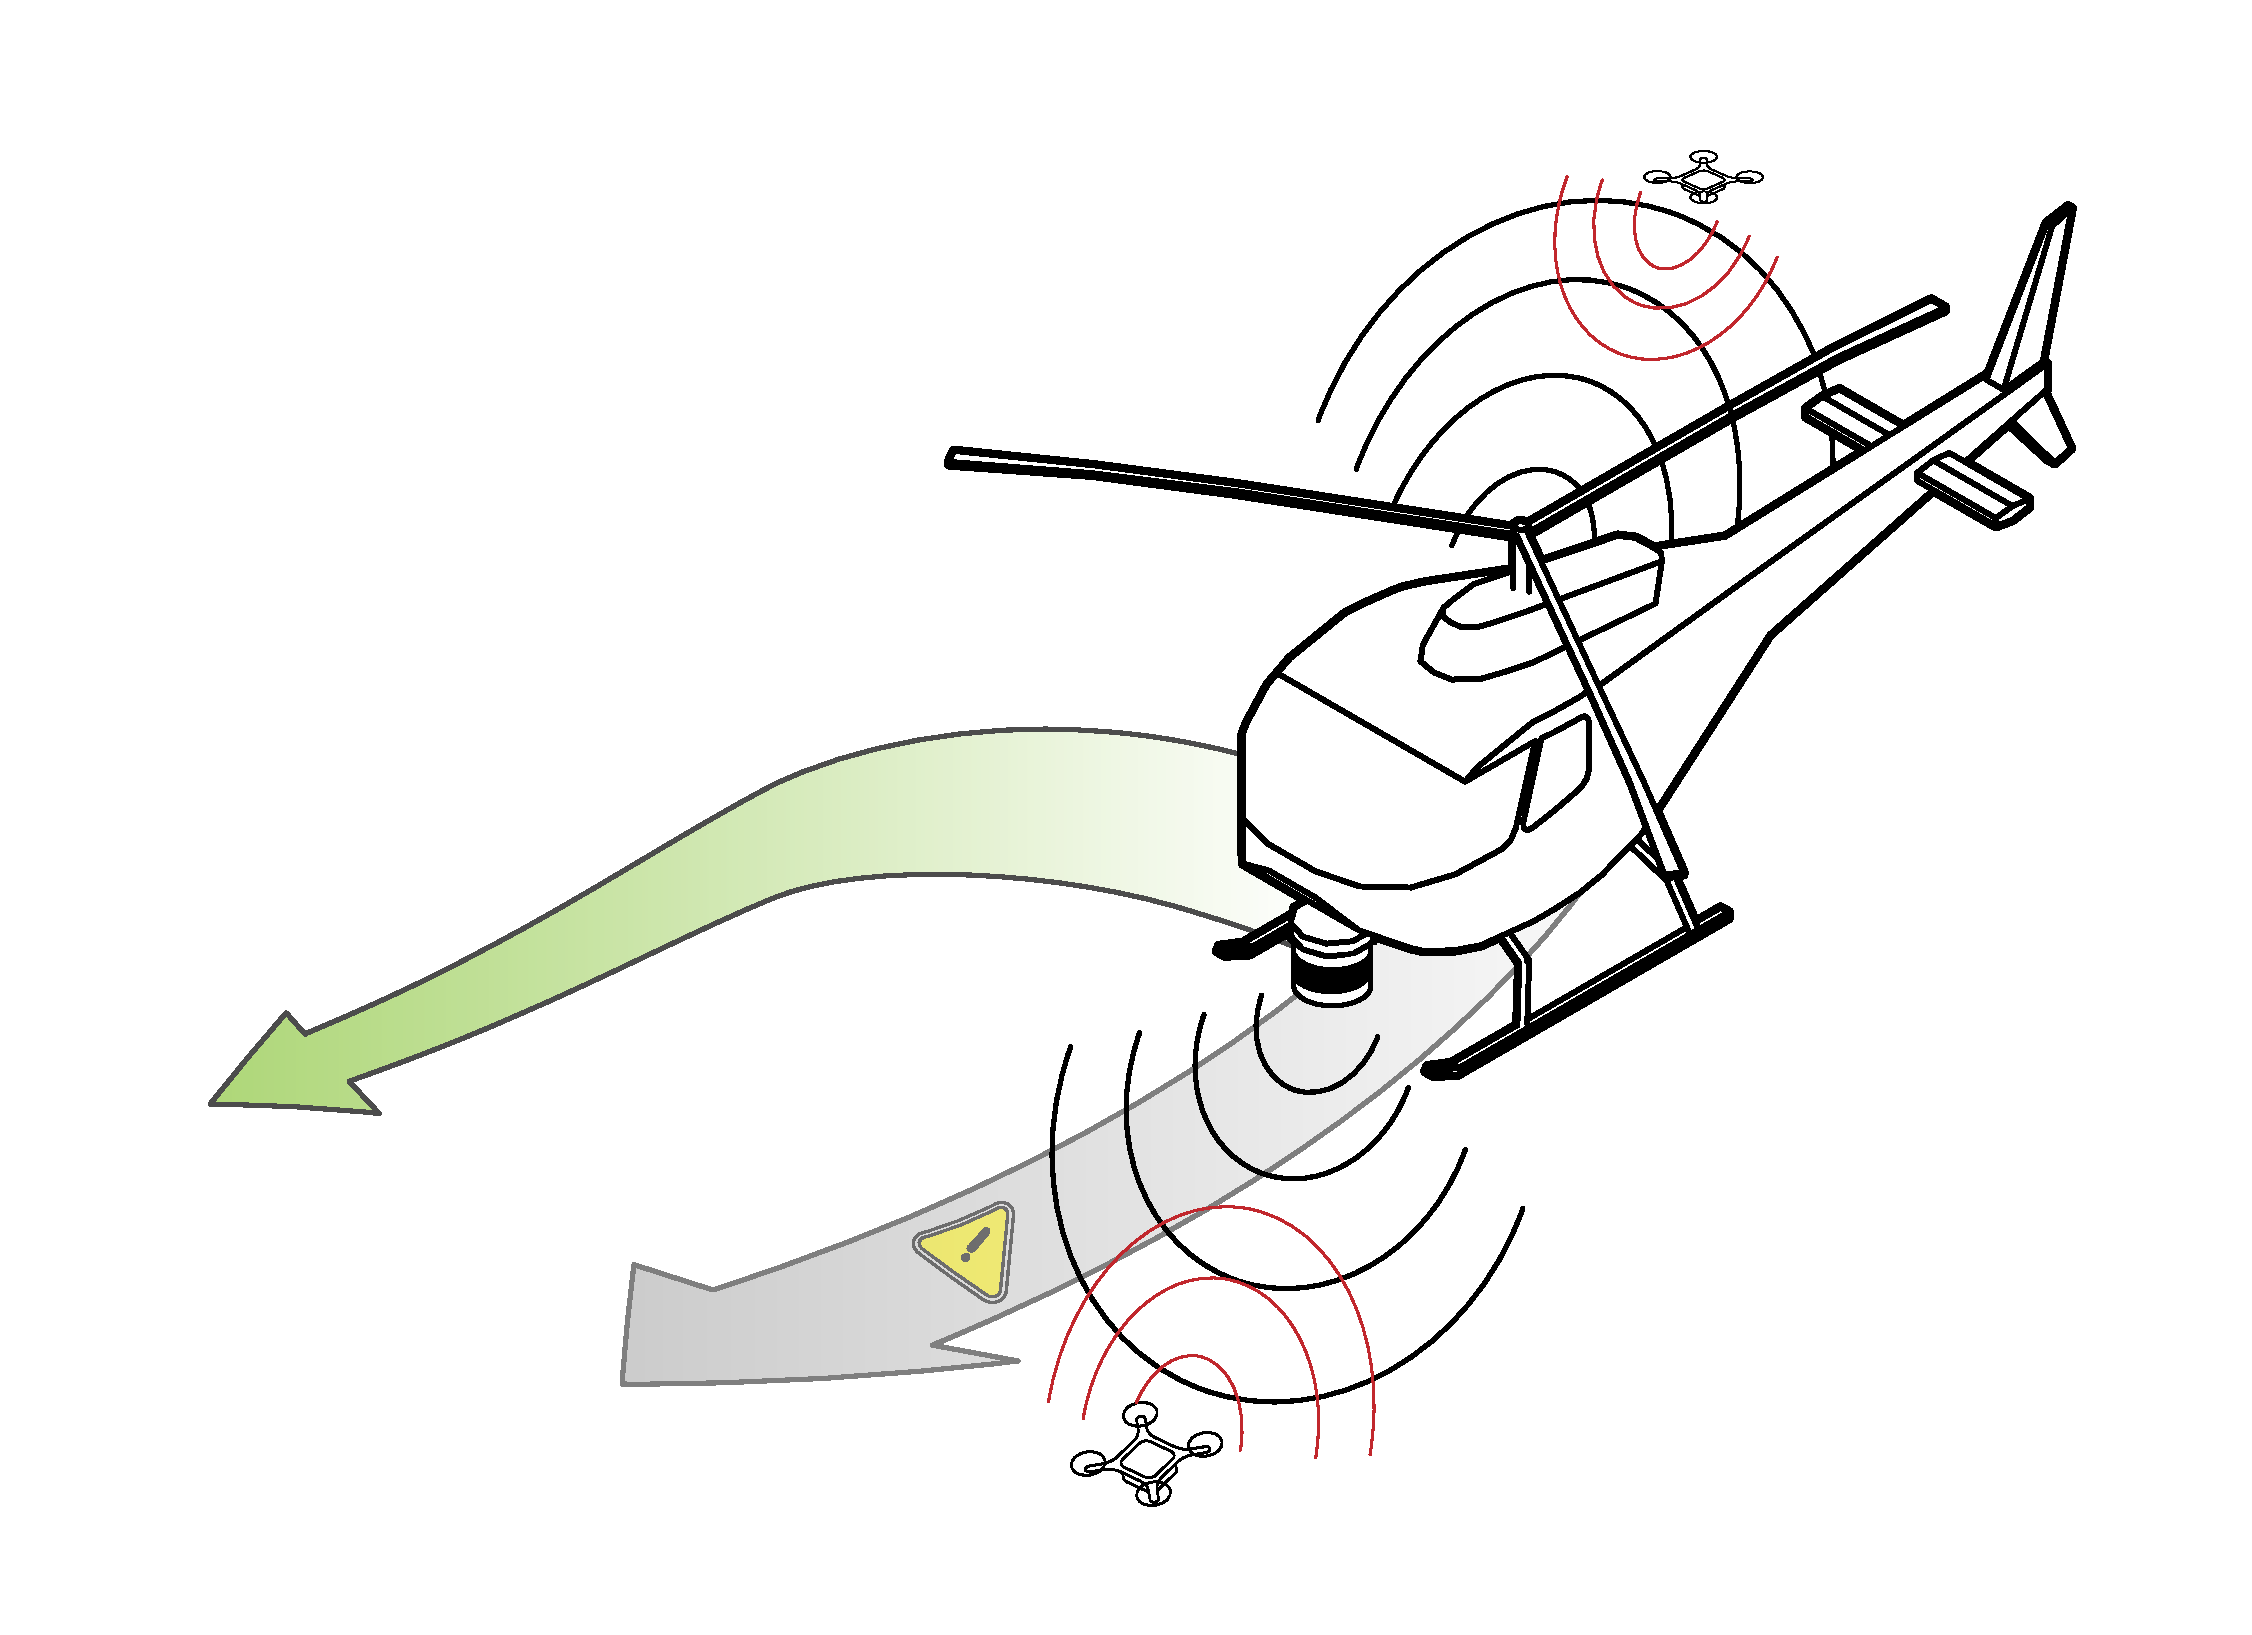
\includegraphics[width=\textwidth]{images/website_bild.pdf}
    \caption{Safety-critical encounter between a helicopter and two small UAVs. The helicopter is equipped with a LiDAR sensor to detect and track the intruding drones. Consequently the initial flight path (gray) is replanned to avoid a collision (green).}
    \label{fig:data_gen_drone}
\end{figure}